\section
{$M^X/M/1$ Queue: Expected Waiting Time}
%{$\mathbf{M^X/M/1}$ Queue: Expected Waiting Time}
\label{sec:mxm1-queue:-expected}


\opt{solutionfiles}{
\subsection*{Theory and Exercises}
\Opensolutionfile{hint}
\Opensolutionfile{ans}
}

It is not always the case that jobs arrive in single units, they can also arrive in batches.
For instance, when a car or a bus arrives at a fast-food restaurant, a batch consists of the number of people in the vehicle.
When the batches arrive as a Poisson process and the individual items within a batch have exponential service times we denote such queueing systems by the shorthand $M^X/M/1$.
In this section, we derive the expressions for the load and the expected waiting time and queue length of the $M^X/M/1$ queue.


Assume that jobs arrive as a Poisson process with rate $\lambda$ and each \emph{job} contains multiple \emph{items}.
Let $A_k$ be the arrival time of job $k$ and $A(t)$ the number of job arrivals up to time $t$.
Denote by $B_k$ the batch size, i.e., the number of items that job $k$ brings into the system.
We assume that $\{B_k\}$ is a sequence of independent discrete random variables each distributed as the generic random variable $B$.
Let the pmf be $\P{B = k} = f(k)$, and $G(k)$ the survivor function.
The service time of each item $\E S = 1/\mu$.
Thus, the average time to serve the entire batch is $\E B \E S$.
 Define the load as
\begin{equation*}
\rho = \lambda \E B/\mu.
\end{equation*}
Henceforth we require that $\rho< 1$.


\begin{exercise}\clabel{ex:l-167} 
Use the renewal reward theorem to explain that work arrives at rate $\lambda \E B$.
\begin{hint}
Observe that the total number of items is given by
\begin{equation*}
Y(t)= \sum_{k=1}^{A(t)} B_k.
\end{equation*}
What should you take for the times $\{T_k\}$? 
\end{hint}
\begin{solution}
Take $T_k = A_k$. Then $X_k = Y(A_k) - Y(A_{k-1}) = B_k$. Hence $X = \lim_{n\to\infty} n^{-1} \lim_{k=1}^n X_k = \E B$. Clearly, $Y = \lim_{t\to\infty} Y(t)/t$ is the arrival rate of work. , The relation $Y=\lambda X$ implies that the arrival rate of work is $\lambda \E B$. 
\end{solution}
\end{exercise}


The aim of the remainder of the section is to derive two cornerstones of queueing theory.
The first is the expected time an item spends in queue:
\begin{equation}\label{eq:32}
\E{W_{Q}} = \frac{1+C_s^2}2 \frac{\rho}{1-\rho} \E B \E S + \frac12\frac\rho{1-\rho}\E S,
\end{equation}
where $C_s^2$ is the SCV of the batch size distribution.
We obtain the second by applying~\cref{eq:wqes}, which evidently also applies here, to the above to find that the expected number of items in the system is
\begin{equation}\label{eq:43}
\E{L} =\frac{\E{W_{Q}}}{\E S} = 
\frac{1+C_s^2}2 \frac{\rho}{1-\rho} \E B + \frac12\frac\rho{1-\rho}.
\end{equation}
Thus, to compute the average number of items in the system, we only need to know the first and second moment (or the variance) of the batch size $B$.



\begin{extra}\clabel{ex:5}
 Show that when the batch size is 1, the expression $\E{L(M^X/M/1)}$, i.e., the system length for the $M^X/M/1$ queue, reduces to
 $\E{L(M/M/1)}$, i.e., the system length for the $M/M/1$ queue. 
\begin{hint}
What is the distribution of the batch size $B$ for the $M/M/1$ queue?
\end{hint}
\begin{solution}
 For the $M/M/1$ queue, each job contains just one item. Thus,
 $B\equiv 1$, hence $\P{B=1}=1$, $\E{B^2}=\E B =1$. Therefore,
 $\E{B_r(M/M/1)}= \rho$, and $\E{L(M/M/1)}=\rho/(1-\rho)$. 
\end{solution}
Realize the importance of such checks.
\end{extra}


\begin{extra}
 What is $\E L$ in case $B_k=3$ always, and $\lambda=1$, $\mu=6$? 
\begin{hint}
Use~\cref{eq:43}. What are $\E{B^2}$, $\E B$ and $\V B$ for this case?
\end{hint}
\begin{solution}
 As $B$ is constant and equal to 3, $\E{B^2}=9$. Hence, $\V B=0$, which implies
 $C_s^2=0$. Also, $\rho=\lambda\E B/\mu=1\cdot 3/6=1/2$. Hence,
 \begin{equation*}
 \E L = \frac 1 2 \frac{1/2}{1-1/2}\cdot 3 + \frac12\frac{1/2}{1-1/2}.
 \end{equation*}
\end{solution}
\end{extra}

\begin{exercise}\clabel{ex:l-168}
 If the batch size is $p$ geometrically distributed, what is $\E L$?
\begin{hint}
$f_k=q^{k-1}p$ with $q=1-p$. Use generating functions to compute $\E B$ and $\E{B^2}$.
\end{hint}
\begin{solution}
 We need $\V B$ and $\E B$. Consider
 \begin{align*}
 M_B(s) 
&= \E{e^{sB}} = \sum_{k=0}^\infty e^{sk} \P{B=k} \\
&= \sum_{k=0}^\infty e^{sk} p q^{k-1} 
= \frac p q \sum_{k=0}^\infty (q e^s)^k = \frac p q \frac1{1-qe^s},\\
 \E B &= M_B'(0) = \left.\frac p q \frac q{(1-q e^s)^2}\right|_{s=0}= \frac p{(1-q)^2} = \frac 1 p,\\
 \E{B^2)} &= M_B''(0) = \frac2{p^2} - \frac1p, \\
 \V B &= \E{B^2} - (\E B)^2 = \frac2{p^2} - \frac1p - \frac1{p^2} = \frac1{p^2}-\frac1p,\\
 C_s^2&= \frac{\V B}{(\E B)^2} = p^2 \left(\frac1{p^2}-\frac1p\right)=1-p,\\
 (1+C_s^2)/2 &= 1-p/2,\\
 \E L &= 
\left(1-\frac p2\right) \frac\rho{1-\rho} \frac 1 p + \frac12\frac\rho{1-\rho}
=\frac\rho{1-\rho} \frac 1 p.
\end{align*}

Can we check this in a simple way? If $\P{B=1}=f_1 = p =1$, then
$\E L=\rho/(1-\rho)$. Thus, we get the result for the $M/M/1$
queue. The result is at least consistent with earlier work.
\end{solution}
\end{exercise}

\begin{exercise}\clabel{ex:64}
 A common operational problem is a machine that receives batches of
 various sizes. Management likes to know how a reduction of the
 variability of the batch sizes would affect the average queueing time.
 Suppose, for the sake of an example, that the batch size 
 \begin{equation*}
 \P{B=1} = \P{B=2} = \P{B=3} = \frac 13.
 \end{equation*}
 Batches arrive at rate 1 per hour.
 The average processing time for an item is $25$ minutes.
 Compute by how much the number of items in the system would decreases if batch sizes were constant and equal to~$2$; hence the load is the same in both cases.
\begin{solution}
 Start with the simple case, $B\equiv 2$. Then $\V{B}=0$ and
 $\E B = 2$. The load is $\rho=\lambda \E B \E S = 1\cdot 2 \cdot 25/60 = 5/6$. Hence,
 \begin{equation*}
 \E{L} = \frac 12 \frac{5/6}{1/6} 2 + \frac 12 \frac{5/6}{1/6} = 5 + \frac52.
 \end{equation*}

Now the other case. $\E{B^2} = (1+4+9)/3 = 14/3$. Hence, $\V B=14/3 - 4=2/3$. Hence, 
\begin{equation*}
C_s^2=\frac{\V B}{(\E B)^2} = \frac{2/3}4 = \frac 16.
\end{equation*}
And thus, 
 \begin{equation*}
 \E{L} = \frac {1+1/6}2 \frac{5/6}{1/6} 2 + \frac 12 \frac{5/6}{1/6} = \frac76 5 + \frac 52.
 \end{equation*}
 If we divide these two answers, we see that the ratio between
 $\E{L}$ for both answers is $10/9$. In other words, we can
 reduce about 10\% of the number of items in the system by working
 in fixed batch sizes. 

Observe how easy it is with these models to get insight into the order of magnitude of queue length reductions or waiting times that can be achieved with changing work habits, such as making batch sizes constant rather than allowing them to vary.
Observe also that it is up to management to decide whether such reductions outweigh any efforts to reduce the variation in batch sizes.

\end{solution}

\end{exercise}


Let us now focus on deriving~\cref{eq:32}.
Assume that an arriving batch joins the end of the queue (if present), and once the queue in front of it has been cleared, it moves in its entirety to the server.
Thus, all items in one batch spend the same time in queue.
Once the batch moves to the server, the server processes the items one after another until the batch is empty.

Suppose that we know $\E{L_S}$, i.e., the average number of items of a batch at the server.

\begin{exercise}\clabel{ex:57}
Show that
 \begin{equation*}
 \E{W_{Q}} = \frac{\E{L_S}}{1-\rho}\E{S}.
 \end{equation*}
\begin{hint}
 Use~\cref{eq:wqes}, $\E{L} = \E{L_{Q}}\E B + \E{L_S}$, where $\E{L_{Q}}$ is the number of batches in queue, and Little's law.
\end{hint}
\begin{solution}
\begin{equation*}
 \E{W_{Q}} 
= \E{L} \E S = (\E{L_{Q}}\E B + \E{L_S})\E S.
\end{equation*}
With Little's law, $\E{L_{Q}} = \lambda \E{W_{Q}}$, hence,
\begin{equation*}
 \E{W_{Q}} 
= \lambda \E S \E B \E{W_{Q}} + \E S \E{L_S} = \rho \E{W_{Q}} + \E S \E{L_S},
\end{equation*}
hence,
\begin{equation*}
 \E{W_{Q}} = \frac{\E{L_S}}{1-\rho}\E S.
\end{equation*}
\end{solution}
\end{exercise}

Clearly, it remains to find an expression for $\E{L_S}$; for this we can again use the renewal reward theorem.
Let $L_S(s)$ be the number of items (of the batch in service) at the server, so that
\begin{equation*}
 Y_i(t) = \int_0^t \1{L_S(s)=i} \d s
\end{equation*}
is the total time up to $t$ there are~$i$ items at the server. 

\begin{exercise}\clabel{ex:l-169}
 Let $\tilde A_k$ be the moment the $k$th batch moves to the server and $D_k$ its departure time.
 Use~\cref{fig:remainingservicetime} to explain that
\begin{equation*}
 \int_{\tilde A_k}^{D_k} \1{L_S(s)=i} \d s = \1{B_k \geq i} S_{k,i},
\end{equation*}
where $S_{k,i}$ is the service time of the $i$th item of this batch. Then show that
\begin{equation*}
 Y_i(D_n) = \sum_{k=1}^n \1{B_k\geq i} S_{k,i}.
\end{equation*}
\begin{hint}
 Observe that $n$ batches have been served at time $D_n$.
\end{hint}
\begin{solution}
Only if $B_k \geq i$ there can be an $i$th item of the batch, and then the time this $i$th item spends at the server is its service time $S_{k,i}$. 

 At the departure time $D_n$ of the $n$th batch, precisely $n$ batches have been served.
 Thus, each batch $k$ with more than $i$ items contributed to $Y_i(D_n)$ with the service time $S_{k,i}$.
\end{solution}
\end{exercise}


\begin{figure}[th]
 \centering
 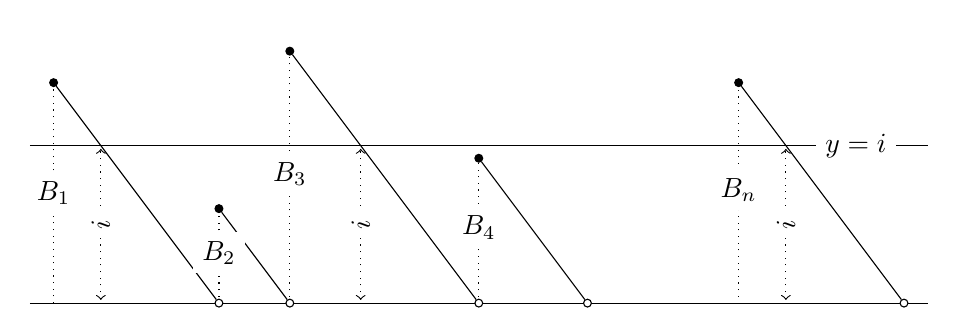
\begin{tikzpicture}[yscale=0.8,xscale=0.6,
 open/.style={shape=circle, fill=white, inner sep=1pt, draw, node contents=},
 closed/.style={shape=circle, fill=black, inner sep=1pt, draw, node contents=}]

 % y = zero line
 \draw (-0.5, 0) -- (18.5, 0); 
 % level crossing
 \draw (-0.5, 2.5) -- (18.5, 2.5) 
 %node[pos=0.65, fill=white, above] {$\sum_{k=1}^n \1{B_k \geq i}$}
 node[pos=0.92, fill=white] {$y=i$};


 \draw node (c1) at (0,3.5) [closed, label={}]
 node (c2) at (3.5,0)[open, label={}]
 (c1) to (c2);
 \draw[dotted] (0,0) -- (0,3.5) node[midway, fill=white] {$B_1$};
 \draw[dotted, <->] (1, 0.05) -- (1, 2.45) node[fill=white, midway, rotate=90] {$i$};


 \draw node (c1) at (3.5,1.5) [closed, label={}]
 node (c2) at (5,0)[open, label={}]
 (c1) to (c2);
 \draw[dotted] (3.5,0.1) -- (3.5,1.5) node[midway, fill=white] {$B_2$};

 \draw node (c1) at (5,4) [closed, label={}]
 node (c2) at (9,0)[open, label={}]
 (c1) to (c2);
 \draw[dotted] (5,0.1) -- (5,4) node[midway, fill=white] {$B_3$};
 \draw[dotted, <->] (6.5, 0.05) -- (6.5, 2.45) node[fill=white, midway, rotate=90] {$i$};

 \draw node (c1) at (9,2.3) [closed, label={}]
 node (c2) at (11.3,0)[open, label={}]
 (c1) to (c2);
 \draw[dotted] (9,0.1) -- (9,2.3) node[midway, fill=white] {$B_4$};

 % end
 \draw node (c1) at (14.5,3.5) [closed, label={}]
 node (c2) at (18,0)[open, label={}]
 (c1) to (c2);
 \draw[dotted] (14.5,0.1) -- (14.5,3.5) node[midway, fill=white ] {$B_n$};
 \draw[dotted, <->] (15.5, 0.05) -- (15.5, 2.45) node[fill=white, midway, rotate=90] {$i$};
 

 % bottom line
 %\draw[<->] (0, -0.6) -- (18, -.6) node[fill=white, midway] {$\sum_{k=1}^n B_k$};
\end{tikzpicture}

\caption{A batch crosses the line $y=i$ iff it contains at least $i$ items.
 Thus, during the service of a batch with $i$ or more items, there is precisely one service of an $i$-th item.}
 \label{fig:remainingservicetime}
\end{figure}


\begin{exercise}\clabel{ex:l-170}
 Now use the renewal reward theorem to show that the (time-average) fraction of time there are~$i$ items at the server is equal to
 \begin{equation*}
 \P{L_S = i} = \lambda \E{S} G(i-1) = \rho \frac{G(i-1)}{\E B}.
 \end{equation*}
Conclude that
\begin{equation*}
 \E{L_S} = \sum_{i=0}^\infty i \P{L_S=i} = \frac{\rho}{\E B} \sum_{i=1}^\infty i G(i-1).
\end{equation*}
\begin{solution}
 By construction, $Y_i(t)/t \to \P{L_S=i}$.
 Let $X_k = Y_i(D_k) - Y_i(D_{k-1})$.
 Then, since the $\{S_{k, i}\}$ are i.i.d. with $\E{S_{k,i}} = \E S$, 
 and the $\{B_k\}$ are i.i.d., we obtain from the previous exercise that $X = \lim_{n\to\infty} n^{-1}\sum_{k=1}^n (S_{k,i} \1{B_{k} \geq i}) = \E{S \1{B\geq i}}$.
 Now $B$ and $S$ are independent by assumption, hence $X = \E{S} \E{\1{B\geq i}} = \E S \P{B\geq i}$.
 The result follows by using rate stability ($\delta = \lambda$) in the renewal reward theorem.
\end{solution}
\end{exercise}

\begin{exercise}\clabel{ex:l-171}
 Brush up the above expression for $\E{L_S}$ to arrive at~\cref{eq:32}.
\begin{solution}
 See~\cref{ex:ER}--\cref{q:batch}.
\end{solution}
\end{exercise}


\begin{extra}\clabel{ex:ER}
 Show that
 \begin{equation*}
 \sum_{i=1}^\infty i G(i-1)= \frac{\E{B^2} + \E B}{2},
\end{equation*}
so that
\begin{equation*}
 \E{L_S} = \rho \frac{\E{B^2}}{2 \E B} + \frac{\rho}{2}.
\end{equation*}

\begin{hint}
 Use~\cref{ex:6} and~\cref{ex:66}.
\end{hint}
\begin{solution}
\begin{equation*}
 \begin{split}
 \sum_{i=1}^\infty i G(i-1) 
&=\sum_{i=0}^\infty (i+1) G(i) 
=\sum_{i=0}^\infty i G(i) +
\sum_{i=0}^\infty G(i)\\
&= (\E{B^2} - \E B + 2\E B)/2.
 \end{split}
\end{equation*}
\end{solution}
\end{extra}


\begin{extra}\label{q:batch}
Finally, 
\begin{equation*}
\rho \frac{\E{B^2}}{2\E{B}} = \frac{1+C_s^2}{2} \rho \E B.
\end{equation*}
\begin{solution}
We have
\begin{align*}
 \frac{\E{B^2}}{\E{B}}
&= \frac{\E{B^2}}{(\E B)^2} \E B 
= \frac{\E{B^2} - (\E B)^2 + (\E B)^2}{(\E B)^2} \E B \\
&= \frac{\V B + (\E B)^2}{(\E B)^2}\E B = (C_s^2+1)\E B.
\end{align*}
\end{solution}
\end{extra}


\begin{exercise}\clabel{ex:l-172}
 Show that $\E{W_Q(M^X/M/1)} \geq \E{W_Q(M/M/1)}$ when the loads are the same.
 What do you conclude?
\begin{hint}
Use~\cref{ex:5,ex:57}
\end{hint}
\begin{solution}
 \begin{equation*}
 \frac{\E{W_Q(M^X/M/1)}}{\E{W_Q(M/M/1)}} = \frac{\E{L_S(M^X/M/1)}}{\E{L_S(M/M/1)}} = \frac{\E{L_S(M^X/M/1)}}{\rho} = 
\frac{\E{B^2}}{2\E B} + \frac 12.
 \end{equation*}
With this we can check whether this condition
 \begin{equation*}
 1\leq \frac{\E{W_Q(M^X/M/1)}}{\E{W_Q(M/M/1)}} = \frac{\E{B^2}}{2\E B} + \frac 12
 \end{equation*}
 is always true. Clearly, it reduces to
\begin{equation*}
\E B \leq \E{B^2}.
\end{equation*}
Multiply this by $\E B$ for reasons to become clear presently to get
\begin{equation*}
(\E B)^2 \leq \E{B^2} \E B.
\end{equation*}
So, the initial inequality is converted to this, and we like to know
whether this always true.


To see this, we can use Jensen's inequality $\phi(\E X) \leq \E{\phi(X)}$ when $\phi$ is convex.
In this case take $\phi(x)=x^2$, so that Jensen's inequality states that $(\E B)^2 \leq \E{B^2}$.
(BTW, note that Jensen's inequality implies that $\V X = \E{X^2} - (\E X)^2\geq 0$.)
Now noting that $B\geq 1$, as a job minimally contains one item, we get
\begin{equation*}
 \begin{split}
(\E B)^2 
&\leq \E{B^2}, \quad{\text{by Jensen's inequality}} \\
&\leq \E{B^2} \E B, \quad{\text{ as } B \geq 1}.
 \end{split}
\end{equation*}
Clearly, this is the inequality we tried to show. As a result,
 \begin{equation*}
 1\leq \frac{\E{W_Q(M^X/M/1)}}{\E{W_Q(M/M/1)}}
 \end{equation*}
for all $B$. 

In conclusion, if work arrives in batches, the average number of jobs
in the system increases, hence the average waiting time increases.
\end{solution}
\end{exercise}




\opt{solutionfiles}{
\Closesolutionfile{hint}
\Closesolutionfile{ans}
\subsection*{Hints}
\input{hint}
\subsection*{Solutions}
\input{ans}
}

%\clearpage

%%% Local Variables:
%%% mode: latex
%%% TeX-master: "../companion"
%%% End:

